\section{eo\-EPReplacement$<$ EOT $>$ Class Template Reference}
\label{classeo_e_p_replacement}\index{eoEPReplacement@{eoEPReplacement}}
EP type of replacement strategy: first add parents to population, then truncate using EP tournament.  


{\tt \#include $<$eo\-Merge\-Reduce.h$>$}

Inheritance diagram for eo\-EPReplacement$<$ EOT $>$::\begin{figure}[H]
\begin{center}
\leavevmode
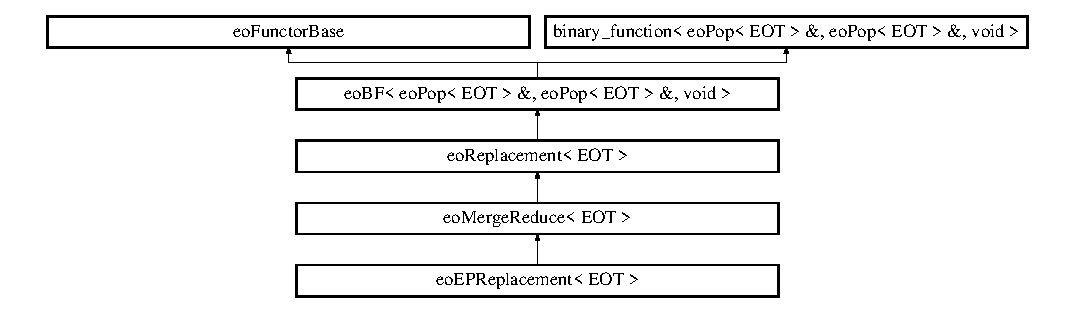
\includegraphics[height=3.76344cm]{classeo_e_p_replacement}
\end{center}
\end{figure}
\subsection*{Public Member Functions}
\begin{CompactItemize}
\item 
{\bf eo\-EPReplacement} (int \_\-t\-Size)\label{classeo_e_p_replacement_a0}

\end{CompactItemize}
\subsection*{Private Attributes}
\begin{CompactItemize}
\item 
{\bf eo\-Plus}$<$ {\bf EOT} $>$ {\bf plus}\label{classeo_e_p_replacement_r0}

\item 
{\bf eo\-EPReduce}$<$ {\bf EOT} $>$ {\bf truncate}\label{classeo_e_p_replacement_r1}

\end{CompactItemize}


\subsection{Detailed Description}
\subsubsection*{template$<$class EOT$>$ class eo\-EPReplacement$<$ EOT $>$}

EP type of replacement strategy: first add parents to population, then truncate using EP tournament. 



Definition at line 102 of file eo\-Merge\-Reduce.h.

The documentation for this class was generated from the following file:\begin{CompactItemize}
\item 
eo\-Merge\-Reduce.h\end{CompactItemize}
